%%
%% This is file `example.tex',
%% generated with the docstrip utility.
%%
%% The original source files were:
%%
%% coppe.dtx  (with options: `example')
%% 
%% This is a sample monograph which illustrates the use of `coppe' document
%% class and `coppe-unsrt' BibTeX style.
%% 
%% \CheckSum{1416}
%% \CharacterTable
%%  {Upper-case    \A\B\C\D\E\F\G\H\I\J\K\L\M\N\O\P\Q\R\S\T\U\V\W\X\Y\Z
%%   Lower-case    \a\b\c\d\e\f\g\h\i\j\k\l\m\n\o\p\q\r\s\t\u\v\w\x\y\z
%%   Digits        \0\1\2\3\4\5\6\7\8\9
%%   Exclamation   \!     Double quote  \"     Hash (number) \#
%%   Dollar        \$     Percent       \%     Ampersand     \&
%%   Acute accent  \'     Left paren    \(     Right paren   \)
%%   Asterisk      \*     Plus          \+     Comma         \,
%%   Minus         \-     Point         \.     Solidus       \/
%%   Colon         \:     Semicolon     \;     Less than     \<
%%   Equals        \=     Greater than  \>     Question mark \?
%%   Commercial at \@     Left bracket  \[     Backslash     \\
%%   Right bracket \]     Circumflex    \^     Underscore    \_
%%   Grave accent  \`     Left brace    \{     Vertical bar  \|
%%   Right brace   \}     Tilde         \~}
%%
\documentclass[grad,numbers]{coppe}
\usepackage{amsmath,amssymb}
\usepackage{hyperref}
\usepackage[utf8]{inputenc}
\usepackage[brazil]{babel}
\usepackage[T1]{fontenc}
\usepackage{graphicx}
\usepackage{placeins}
\usepackage{textgreek}
\usepackage{amsmath}
\usepackage{amssymb}
\usepackage{enumitem}


\makelosymbols
\makeloabbreviations

\begin{document}
  \title{Desenvolvimento de um equipamento de baixo custo para medição de parâmetros da frequência respiratória com aplicação em neurociência comportamental humana.}
  \foreigntitle{low cost equipment designed to measure respiratory frequency parameters applied to human behavioral neuroscience}
  \author{Bruno Gomes}{Reis}
  \advisor{Prof.}{Carlos José Ribas}{D'Avila}{M.Sc.}
  \advisor{Prof.}{Tiago Arruda}{Sanchez}{Ph.D.}
  %\advisor{Prof.}{Nome do Terceiro Orientador}{Sobrenome}{D.Sc.}

  \examiner{Prof.}{Nome do Primeiro Examinador Sobrenome}{D.Sc.}
  \examiner{Prof.}{Nome do Segundo Examinador Sobrenome}{Ph.D.}
  \examiner{Prof.}{Nome do Terceiro Examinador Sobrenome}{D.Sc.}
  \examiner{Prof.}{Nome do Quarto Examinador Sobrenome}{Ph.D.}
  \examiner{Prof.}{Nome do Quinto Examinador Sobrenome}{Ph.D.}
  
  
  
  \department{EEC}% Confira a tabela a seguir para saber como preencher o comando \department de acordo com seu curso (Graduação - Poli) ou programa (Pós-Graduação - COPPE).
  
  %%%%%% Para alunos da POLI %%%%%%
  
  %% Course											Option
  %% Engenharia Ambiental                             EA
  %% Engenharia Civil                                 ECV
  %% Engenharia de Computação e Informação            ECI
  %% Engenharia de Controle e Automação               ECA
  %% Engenharia de Materiais                          EMAT
  %% Engenharia de Petróleo                           EPT
  %% Engenharia de Produção                           EPR
  %% Engenharia Eletrônica e de Computação            EEC
  %% Engenharia Elétrica                              EET
  %% Engenharia Mecânica                              EMC
  %% Engenharia Metalúrgica                           EMET
  %% Engenharia Naval e Oceânica                      ENO
  %% Engenharia Nuclear                               ENU
  
  
  %%%%%% Para alunos da COPPE %%%%%%
  
  %% Program											Option
  %% Engenharia Biomédica								PEB
  %% Engenharia Civil									PEC
  %% Engenharia Elétrica								PEE
  %% Engenharia Mecânica								PEM
  %% Engenharia Metalúrgica e de Materiais				PEMM
  %% Engenharia Nuclear									PEN
  %% Engenharia Oceânica								PENO
  %% Planejamento Energético							PPE
  %% Engenharia de Produção								PEP
  %% Engenharia Química									PEQ
  %% Engenharia de Sistemas e Computação				PESC
  %% Engenharia de Transportes							PET
  
  
  
  
  
  
  \date{08}{2019}

  \keyword{Behavioral Neuroscience}
  \keyword{Respiratory Frequency }
  \keyword{Engenharia Eletrônica e de Computação}

  \maketitle

  \frontmatter
  
  \makecatalog
  
  \dedication{Dedico este trabalho às minhas famílias de sangue e coração.}

  \chapter*{Agradecimentos}

  Gostaria de agradecer a todos.

  \begin{abstract}
  	
	O RESUMO SERÁ ESCRITO AQUI
	
	
%	...Nesse desenvolvimento, utilizamos um termistor como sensor a fim de obter informações sobre a frequência respiratória através da variação de temperatura, causada pelo contato do sensor com o fluxo de ar provocado inspiração e expiração humana...
        
  \end{abstract}

  \begin{foreignabstract}

  In this work, we present ...

  \end{foreignabstract}

  \tableofcontents
  \listoffigures
  \listoftables
  \printlosymbols
  \printloabbreviations

  \mainmatter
%  \doublespacing
  
    \chapter{Introdução}
  
  \section{Tema}
  
  O tema do trabalho é o desenvolvimento de um dispositivo que realize a medição da frequência respiratória dentro de uma faixa sensível para respostas psicofisiológicas. Este dispositivo deve possibilitar o monitoramento e a extração de dados que auxiliarão em estudos os quais correlacionam alguns parâmetros da frequência respiratória com funções psicofisiológicas, como aquelas observadas sob alterações cognitivas, emocionais, sob estresse  doenças mentais.
  
  \section{Delimitação}
  
  O objeto de estudo é o desenvolvimento de um protótipo capaz de mensurar comportamentos respiratórios tais quais a frequência de inspiração e expiração, para, a partir desse, analisar a viabilidade de desenvolvimento de um equipamento com baixo custo voltado ao uso científico. As medições terão como finalidade a obtenção de dados, referentes à frequência respiratória do paciente, a serem utilizados em experimentos que vinculem comportamentos saudáveis e suas variantes clínicas à respiração humana. O estudo, limita-se à obtenção desses dados, não abrangendo, a priori, interpretações acerca das correlações obtidas em eventuais medições realizadas, além de possuir, em princípio, finalidade meramente científica, sem conter qualquer estudo sobre viabilidade comercial de produtos que venham a ser desenvolvidos.
  
  \section{Justificativa}
 
   Segundo Sebastião Gusmão \cite{gusmao2004historia}, a medicina como ciência, baseada na interpretação natural da doença e não em magia e empirismo, como ocorria na medicina arcaica, tem sua origem no século V a.C com Hipócrates (c. 460-375 a.C). Desde então, análises e estudos sobre o funcionamento do corpo humano, bem como as interações deste com o meio ambiente, vêm sendo realizados em constante evolução. Hoje, sabe-se que o organismo humano é composto de diversas partes que, em conjunto, garantem o seu funcionamento adequado. O corpo é, portanto, um sistema complexo no qual atuam diversas variáveis. Sendo assim, grande parte dos estudos científicos atuais voltam seus métodos e análises ao estudo dos parâmetros que possuem influências para o bom ou mal funcionamento do organismo. Atualmente, sabe-se que diversas doenças psicofisiológicas produzem variações no funcionamento normal do corpo, como alterações na produção de determinados hormônios, no batimento cardíaco, na pressão arterial ou na concentração de $CO_2$ no sangue. 
   
   Estudos recentes demonstram que é possível por exemplo, induzir pânico em ratos apenas alterando a concentração de $O_2$ ou de $CO_2$ do ar por eles respirado \cite{spiacci2015serotonin} \cite{spiacci2018panic}. A respiração humana é, assim como nos ratos, o processo natural responsável pela troca do $CO_2$ com o $O_2$.    
    
   Ao realizar uma análise de correspondência (correlação, regressão, inferência etc.) entre determinado comportamento biológico e algum quadro clínico específico, o 		pesquisador necessita realizar, de alguma maneira, a mensuração das variáveis que compõem o comportamento com acurácia e significado preditivo para a sensibilidade e a especificidade dos resultados. Nesse sentido, o desenvolvimento de um equipamento de baixo custo capaz de coletar dados referentes ao comportamento respiratório torna-se parte essencial à evolução do estudo científico. 
      
   Munido dessa motivação, neste trabalho, apresentam-se estudos para viabilidade do desenvolvimento de uma tecnologia com baixo custo capaz de monitorar o comportamento do fluxo respiratório de pacientes, servindo então como base para estudos científicos na área de neurociência comportamental. 
 
  \section{Objetivos}
  
	O objetivo geral deste estudo é, então, desenvolver um protótipo de equipamento capaz de realizar a aquisição de dados referentes à frequência respiratória em humanos, incluindo parâmetros que possam ser utilizados em pesquisas neurocientíficas. Desta forma, tem-se como objetivos específicos: (1) Realizar a mensuração da frequência respiratória (2) desenvolver os métodos de medida da frequência respiratória para extrair suas variantes no domínio do tempo e da frequência; e (3) Possibilitar a exportação dos dados para análises futuras.
  
  
  \section{Metodologia}

	A priori, a medição da frequência respiratória seria obtida indiretamente pela variação da temperatura do ar próximo à narina do paciente, uma vez que, em um ambiente controlado, o ar inalado possui uma temperatura inferior à do ar exalado. Contudo, no decorrer do desenvolvimento, foi observado que seria inviável a realização desse tipo de medição devido à baixa variação entre essas duas temperaturas e à velocidade de resposta necessária para a obtenção dos dados de forma confiável utilizando equipamentos de baixo custo. Para contornar esse problema, foi utilizada a propriedade de autoaquecimento do termistor, que passou a ser utilizado como um sensor de fluxo. Ou seja, o sistema não mais tenta inferir a frequência respiratória com base no aumento da temperatura ambiente ocasionada pela saída de ar quente do corpo humano, ao contrário, ele aplica uma corrente muito alta no sensor forçando-o a atingir por conta própria uma temperatura ainda maior em seu estado permanente e, no momento de seu encontro com qualquer fluxo de ar resultante da respiração humana, o sensor registra uma alta queda de temperatura, registrando, de forma mais nítida o momento da ação respiratória.

	O termistor é um resistor variável à temperatura, escolhido principalmente por suas propriedades de autoaquecimento e pela variação exponencial de sua resistência em relação à mudança na temperatura, contrário a grande parte dos demais sensores que possuem uma relação linear entre essas variáveis. Trabalhar com um sensor de cuja curva característica é exponencial facilita detecções de pequenas variações na temperatura, gerando grandes mudanças na resistência, em contrapartida, adiciona complexidade ao sistema dado que trabalhar com relações lineares é, em geral, mais simples. A escolha do termistor é portanto perfeita porque sua contrapartida sequer implica em complicações para o sistema deste trabalho, dado que, em princípio, não interessa uma medição precisa da temperatura, mas sim o registro dos eventos de inspiração e expiração.
	
	O sistema é composto de uma fonte capaz de entregar ao sensor corrente suficiente para que este entre em estado de autoaquecimento e atinja uma temperatura alta o suficiente para se tornar sensível à variação provocada pelos fluxos de ar, um circuito regulador responsável por filtrar sinais indesejados e controlar a corrente de entrada no termistor, um microcontrolador que irá realizar as medições e um software capaz de exportar os dados para que esses possam ser tratados e estudados em suas aplicações.  

  \section{Organização do Trabalho}
  Nos próximos capítulos serão apresentados em mais detalhes as aplicações, o desenvolvimento e os resultados obtidos com esse trabalho, organizados da seguinte forma:
  
  O capítulo 2 apresentará a motivação para o desenvolvimento do equipamento, as aplicações no campo da medicina e um resumo do funcionamento fisiológico da respiração humana. 
  
  O capítulo 3 tratará sobre desenvolvimento do sistema, hardware e software bem como o raciocínio por trás da arquitetura.
  
  O capítulo 4 apresentará a lista de materiais utilizados no projeto
  
  O capítulo 5 será destinado à conclusão desse projeto, com o protótipo construído no último ciclo de desenvolvimento, limitações encontradas ao longo das etapas e também possíveis melhorias para trabalhos futuros.
 

  \chapter{Motivação}
  
\section{Fisiologia da Respiração} \label{sec:fisiologiadarespiracao}

	A respiração é, em resumo, um ato automático do qual o controle é exercido por centros respiratórios no tronco encefálico, onde são produzidos impulsos neuronais para os músculos respiratórios. 
	
	A inspiração possui como músculo principal o diafragma, que se contrai, desce e expande a cavidade torácica, comprimindo então o conteúdo abdominal e empurrando para fora a parede abdominal. Concorrentemente, os músculos da caixa torácica também expandem o tórax, em especial, os músculos escalenos que percorrem das vértebras cervicais às duas primeiras costelas e os músculos intercostais paraesternais, que possuem um trajeto desde o externo até as costelas. Na medida em que o tórax se expande, a pressão intratorácica diminui, deslocando o ar da árvore traqueobrônquica para os alvéolos, preenchendo os pulmões em expansão. O oxigênio é então difundido para os capilares pulmonares adjacentes, enquanto o dióxido de carbono sai do sangue para os alvéolos.
	
	Quando ocorre a expiração, a parede torácica bem como os pulmões retraem-se, o diafragma relaxa, elevando-se passivamente, enquanto o ar flui para fora do corpo.
	
	Em estado normal, a respiração é tranquila, audível próximo à boca, sendo possível observar apenas os movimentos abdominais com facilidade. Contudo, durante a prática de atividade física, ou em decorrência de determinadas doenças, faz-se necessário um esforço respiratório adicional, recrutando músculos acessórios e demandando ainda mais esforço dos músculos abdominais, que passa a auxiliar também na expiração.
	
\section{Padrões Respiratórios} \label{sec:padroesrespiratorios}

	A faixa de frequência padrão para adultos normais é de, aproximadamente, 14 à 20 incursões por minuto e até 44 em lactantes. Em sua normalidade, a inspiração e expiração possuem o mesmo tempo e amplitude, sendo intercalados por uma leve pausa. No momento em que uma dessas características é modificada, surgem os ritmos respiratórios anormais, tais quais a respiração de Cheyne-Stokes, respiração de Biot, respiração de Kussmaul e respiração suspirosa.
	
	Respiração de Cheyne-Stokes: Frequentemente causada por insuficiência cardíaca, hipertensão intracraniana, acidentes vasculares cerebrais e traumatismos cranioencefálicos. Caracteriza-se por uma fase de apneia seguida de incursões inspiratórias cada vez mais profundas até atingir um máximo e, em seguida, decrescer até uma nova pausa. Esse comportamento ocorre devido a variações da tensão de $O_2$ e $CO_2$ no sangue. O excesso de $CO_2$ durante o período de apneia obriga os centros respiratórios a enviar estímulos mais intensos, resultando em um aumento da amplitude dos movimentos respiratórios, em consequência, haverá uma maior eliminação de $CO_2$ fazendo com que a concentração deste no sangue decaia. Após essa queda, os centros respiratórios recebem o comando inverso, enviando estímulos menores e diminuindo a amplitude dos movimentos respiratórios até que aumente novamente a concentração de $CO_2$ no sangue e o ciclo se repita.
	
	Respiração de Biot (ou atáxica): As causas dessa respiração são similares às da respiração de Cheyne-Stokes, porém, no ritmo de Biot, a respiração possui duas etapas, uma de apneia seguida de outra com movimentos respiratórios anárquicos quanto ao ritmo e à amplitude. Esse padrão respiratório quase sempre indica um grave comprometimento cerebral.
	
	Respiração de Kussmaul: Costuma ser causada pela acidose (diminuição do PH sanguíneo para menos de 7,35[aumento de H+]), principalmente a diabética. O padrão respiratório é composto de quatro fases: Inspirações ruidosas, gradativamente mais amplas, alternada com inspirações rápidas e de pequena amplitude; Apneia em inspiração; Expirações ruidosas, gradativamente mais profundas, alternadas com inspirações rápidas e de pequena amplitude;	
	E apneia em expiração.
	
	Respiração suspirosa: Normalmente, pode ser traduzida em tensão emocional e ansiedade. Seu padrão ocorre quando o paciente executa uma série de movimentos inspiratórios de amplitude crescente, seguidos de uma expiração breve e rápida.
	
	Além desses padrões respiratórios, existem diversos outros padrões observados (como a Taqpineia, Bradpneia, Respiração obstrutiva e Hiperpneia) que possuem correlação com patologias ou alterações emocionais e, portanto, existe um vasto campo de estudo acerca desse tema.
	
\section{Aplicação do equipamento}

	Motivado pela parceria com o "Laboratório de Neuroimagem e Psicofisiologia", situado no Hospital Universitário Clementino Fraga Filho, ocorre o desenvolvimento deste projeto. Orientado principalmente a estudos na área de neurociência comportamental, o desenvolvimento do equipamento visa trazer mais insumos às análises realizadas nos diversos projetos existentes no laboratório. Conforme mencionado na sessão \ref{sec:padroesrespiratorios}, existem diferentes padrões respiratórios já observados entre os quais se é possível obter uma relação de correlação com patologias e alterações emocionais e comportamentais. Por derradeiro, a existência de um equipamento capaz de obter dados referentes ao comportamento respiratório transcreve-se em um ganho à neurociência comportamental pelo qual este projeto se justifica.
  

  \chapter{Desenvolvimento}
  
\section{O funcionamento do termistor}
 
	O termistor é um resistor variável à temperatura, característica pela qual seu nome é inspirado (temperatura + resistor), geralmente compostos por uma liga que contém cerâmica e outros polímeros. Suas aplicações mais habituais costumam acontecer em circuitos de monitoramento e controle de temperatura ou como limitador de corrente de partida. São separados, basicamente, em duas categorias:
	\begin{itemize}
		\item NTC (Negative Temperature Coefficient): São termistores que diminuem a sua resistência à medida em que a temperatura aumenta; E
		\item PTC (Positive Temperature Coefficient): Termistores que aumentam a sua resistência diretamente com o aumento da temperatura.
	\end{itemize}
	
	\subsection{A equação de Steinhart–Hart}
	
		A curva de variação da resistência de um termistor em função de sua temperatura pode ser descrita pela equação de Steinhart–Hart\ref{eq:steinharthart} em sua forma inversa \ref{eq:steinharthartinverted}. A característica logarítmica da resposta com que a resistência varia em função da variação de temperatura (figura \ref{fig:curva_termistor}) é, em grande parte das vezes, uma das principais vantagens do seu uso, visto que pequenas variações na temperatura provocam grandes alterações na resistência, fazendo com que o sensor seja mais suscetível a detectar pequenas mudanças na temperatura.
		
		
		\begin{equation}\label{eq:steinharthart}
		\dfrac{1}{T} = a + b\ln{(R)} + c(\ln{(R)})^3
		\end{equation}
		Sendo:
		\begin{itemize}
			\item T: Temperatura em Kelvins;
			\item R: Resistência em ohms ($\Omega$);E
			\item a,b e c: Coeficientes de Steinhart–Hart, que são variáveis conforme o tipo de material e a construção do termistor.		
		\end{itemize}
		
		
		\begin{equation}\label{eq:steinharthartinverted}
			\begin{aligned} [left]
			& R = \exp{(\sqrt[3]{\beta - \dfrac{\alpha}{2}} - \sqrt[3]{\beta + \dfrac{\alpha}{2}})},
			\\
			& \alpha = \dfrac{1}{c}(a - \dfrac{1}{T}),
			\\
			& \beta = \sqrt{(\dfrac{b}{3c})^3 + (\dfrac{\alpha}{2})^2}
			\end{aligned}
		\end{equation}
	
	
		\begin{figure}[h!]
			\begin{center}
				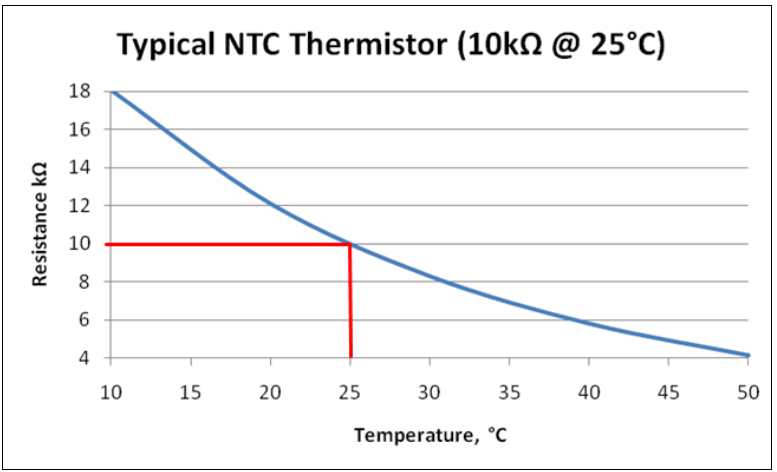
\includegraphics[width=1\linewidth]{images/curva_termistor.png}
				\caption[Curva de resposta típica em termistores NTC de 10k$\Omega$]{Curva de resposta típica em termistores NTC de 10k$\Omega$\footnotemark}
				\label{fig:curva_termistor}
			\end{center}
		\end{figure}
	
		\footnotetext{Fonte: http://www.squids.com.br/arduino/index.php/projetos-arduino/projetos-squids/basico/159-projeto-42-comparando-sensores-de-temperatura-ntc-10k-dht11-e-lm35}


	\subsection{O efeito de Autoaquecimento}

		Como toda resistência, o termistor dissipa energia elétrica na forma de calor. Portanto, ao aplicar uma corrente no sensor, é induzido um efeito de autoaquecimento. A relação da potência elétrica dissipada é dada pela equação \ref{eq:potenciaeletrica} e a relação entre potência e temperatura pode ser obtida através da equação \ref{eq:potenciatermica}. Fazendo $P_E = P_T$, é possível chegar à equação \ref{eq:temperaturacomautoaquecimento}. 
		
		\begin{equation}\label{eq:potenciaeletrica}
			P_E = I.V
		\end{equation}
		sendo:
		\begin{itemize}
			\item $P_E$: Potência elétrica dissipada;
			\item $I$: Corrente elétrica;E
			\item $V$: Tensão entre os terminais.
		\end{itemize}

		\begin{equation}\label{eq:potenciatermica}
			P_T = K(T_{(R)} - T_0)
		\end{equation}
		sendo:
		\begin{itemize}
			\item $P_T$: Potência;
			\item $K$: Fator de dissipação do termistor;
			\item $T_{(R)}$: Temperatura em função da resistência;E
			\item $T_0$: Temperatura ao redor do termistor.
		\end{itemize}
		
		\begin{equation} \label{eq:temperaturacomautoaquecimento}
			T_0 = T_{(R)} - \dfrac{V^2}{K.R}
		\end{equation}
		

\section{A evolução do circuito}
 
Valendo-se da propriedade logarítmica do termistor, uma pequena variação de temperatura ambiente ocasionada pelo processo de expiração ocasionaria uma mudança exponencial no valor da resistência. Por esse motivo, na origem do projeto, era esperada uma medição simples, obtida através da variação de tensão em um divisor resistivo composto por um termistor e uma resistência padrão(Figura: \ref{fig:divisorResistivo}). Contudo, devido alguns contratempos práticos, diversas mudanças fizeram-se necessárias. 
 

 
Uma das principais limitações para o desenvolvimento do projeto deve-se à dificuldade na aquisição dos componentes eletrônicos que, quando comprados via internet, necessitavam de um tempo para entrega relativamente alto e, para a compra realizada diretamente na loja física, existe uma limitação na variedade de lojas especializadas na cidade do Rio de Janeiro. Outra complicação relevante é referente à ausência de datasheet, que não é informado no momento da compra e torna-se impossível inferir qual é o datasheet correto apenas observando o componente, que é muito pequeno, sem qualquer informação sobre o fabricante ou o modelo. Dadas essas condições iniciais, foi construído o primeiro divisor resistivo apenas com base na informação de que o sensor adquirido tratava-se de um termistor NTC (do inglês Negative Temperature Coefficient) com resistência em temperatura ambiente de $10K\Omega$. Foi utilizada uma fonte de alimentação comercial de $12V$ e utilizado diversos valores entre $10K\Omega$ e $330\Omega$ para a resistência $R2$, contudo para nenhum valor de $R2$ era observada qualquer alteração de tensão na medida em que o ar era exalado próximo ao sensor, contrariando ao que era esperado, dado que a queda de tensão em cima do termistor deve ser variável junto à alteração na resistência.
 
\begin{figure}[h!]
	\begin{center}
 		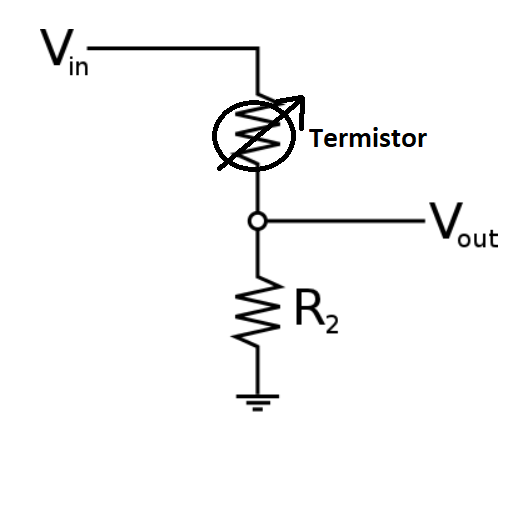
\includegraphics[width=0.5\linewidth]{images/divisor_resistivo.png}
 		\caption{Divisor Resistivo}
 		\label{fig:divisorResistivo}
 	\end{center}
\end{figure}
 
A lei de resfriamento de newton (\ref{eq:resfriamento}) indica que a taxa com que um corpo perde calor é proporcional à diferença de temperatura entre o corpo e o meio  no qual ele se encontra. Valendo-se desse princípio, nota-se que uma baixa diferença de temperatura resultaria em um maior tempo de resposta do sensor. Portanto, para contornar o problema obtido, o circuito foi ajustado para utilizar a propriedade de autoaquecimento do termistor (\ref{eq:autoAquecimento}). 
 
  
\begin{equation} \label{eq:resfriamento}
	\dfrac{dQ}{dt} = h.A.(T(t) - T_{env}) = h.A \Delta T(t)	
\end{equation}
Onde:
\begin{itemize}[label=]
	\item $Q$: Energia térmica
	\item $t$: Tempo
	\item $h$: Coeficiente de transferência de calor
	\item $A$: Área de transferência de calor
	\item $T$: Temperatura do objeto
	\item $T_{env}$: Temperatura do ambiente
\end{itemize}
 
\begin{equation} \label{eq:autoAquecimento}
	T_0 = T(R) - \dfrac{V^2}{KR}
\end{equation}
Onde:
\begin{itemize}[label=]
	\item $T_0$: Temperatura do meio
 	\item $T(R)$: Temperatura do termistor em função de sua resistência
 	\item $V$: Diferença de potencial entre os terminais do termistor
 	\item $K$: Fator de dissipação do termistor
 	\item $R$: Resistência
\end{itemize}
 
 
 
Ao aplicar uma alta corrente no sensor, é induzido então um aumento na temperatura deste. Em decorrência desse aumento, é possível observar uma maior diferença de temperatura entre o sensor e o fluxo de ar e, por conseguinte, uma maior taxa para transferência de calor e um menor tempo de resposta por parte do termistor. Contudo, para atingir uma faixa de temperatura sensível, capaz de gerar uma resposta visível ao expor o sensor à respiração, o circuito necessita de uma tensão elevada, acima das entregues por fontes comerciais padrão, que costumam variar entre $5V$ e $12V$, gerando a necessidade de projetar um retificador de tensão capaz de converter a tensão de corrente alternada entregue pela rede elétrica residencial em uma tensão contínua alta o suficiente para fornecer ao termistor a corrente demandada.
 
Realizando testes de bancada, com um gerador de tensão variando de $0V$ à $30V$ e uma resistência de $330\Omega$ em série com o termistor, foi possível atingir uma temperatura sensível ao sopro, entretanto, ao aplicar uma tensão em torno de $22V$, o sensor demorava um tempo considerável para aquecer novamente, tornando-o inviável para medir o comportamento respiratório dada a frequência do sopro em uma respiração normal. Aumentando a tensão para $28V$, já era possível observar uma atenuação considerável na queda constante da temperatura dado que o termistor era capaz de se aquecer mais rápido. O problema gerado por esse aumento de tensão deve-se ao fato de que, quanto maior é a corrente, maior é o autoaquecimento e, quanto maior a temperatura, menor é a resistência, gerando um aumento ainda maior na corrente passante que, por sua vez, aumenta ainda mais a temperatura até que o sensor atingia um patamar no qual queimava, caso não houvesse nenhum sopro forçando a temperatura a diminuir. 
 
Se por um lado, o aumento da tensão era importante para que a temperatura não decaísse constantemente ao iniciar a medição respiratória, por outro, o sistema precisava ser protegido para que a corrente não atingisse um determinado patamar que danificasse o componente. O ajuste mais simples para regular a corrente em um componente costuma ser adicionar uma resistência em série, diminuindo a corrente por uma mera consequência da lei de ohm (\ref{eq:leideohm}). Contudo, por se tratar de uma resistência variável, a tensão necessária para o aquecimento do termistor em seu estado inicial era maior que a tensão necessária para mantê-lo abaixo de um patamar seguro após a diminuição de sua resistência pelo efeito do autoaquecimento. Foi pensado então em um circuito de controle não linear (Figura: \ref{fig:circuitoRealimentado}), que, em teoria, forneceria uma alta tensão para o termistor até que sua resistência variasse e a corrente passante atingisse um patamar determinado. 
  
\begin{equation} \label{eq:leideohm}
	V = R.I
\end{equation}
Onde:
\begin{itemize}[label=]
  	\item $V$: Tensão
  	\item $R$: Resistência
  	\item $I$: Corrente
\end{itemize}

\begin{figure}[h!]
	\begin{center}
		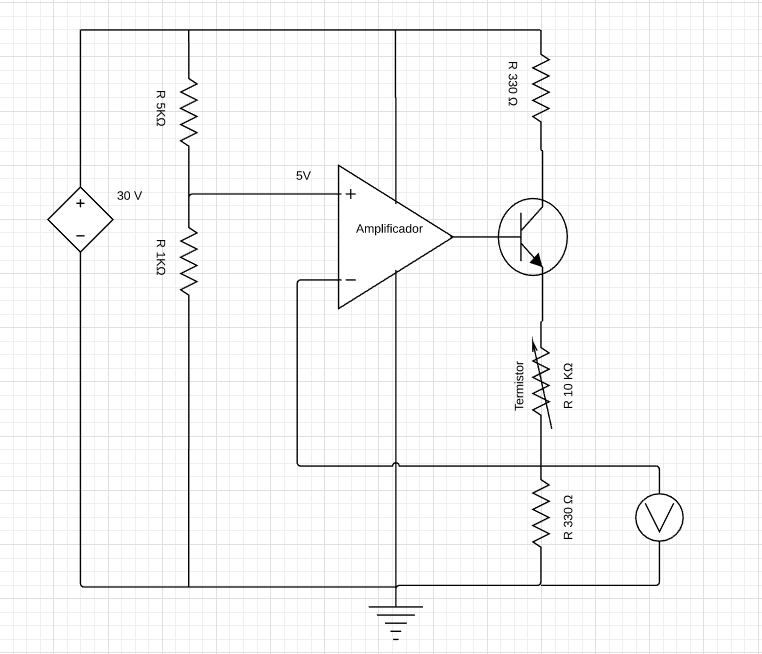
\includegraphics[width=1\linewidth]{images/Circuito_de_controle.png}
		\caption{Circuito de Controle}
		\label{fig:circuitoRealimentado}
	\end{center}
\end{figure}

O comportamento esperado para o circuito de controle seria o seguinte: O amplificador operacional iria ajustar a tensão de saída na tentativa de igualar as tensões nos dois terminais de entrada, sendo assim, no momento inicial, quando a tensão no terminal de entrada negativo é igual a zero e a do terminal positivo é igual a $5V$, o amplificador aumenta sua saída fazendo com que o transistor entre em saturação e conduza uma corrente no emissor praticamente igual à de referência no coletor, na medida em que a resistência do termistor diminui pelo efeito de autoaquecimento, a tensão de saída aumenta até que esta se iguale à do terminal positivo, ao atingir esse patamar, o transistor saí da zona de saturação e o sistema trabalha pra manter a tensão de saída constante. No momento em que o sensor entra em contato com o fluxo de ar, a resistência do termistor aumenta, diminuindo a tensão na saída e estimulando o sistema de controle a saturar o transistor e induzir o efeito do autoaquecimento no sensor. Após quantizar a tensão da saída através de um microcontrolador, foi possível traçar o gráfico da figura \ref{fig:RespostaCircuitoRealimentado}, no qual aparece nítida a resposta do sistema ao submeter o sensor a um fluxo de ar. Entretanto, ao expor o sensor a um período prolongado de exposição à respiração humana, foi possível observar que o efeito do resfriamento contínuo continuava a ser reproduzido (gráfico da figura \ref{fig:RespostaCircuitoRealimentadoLongoPrazo}).


\begin{figure}[h!]
	\begin{center}
		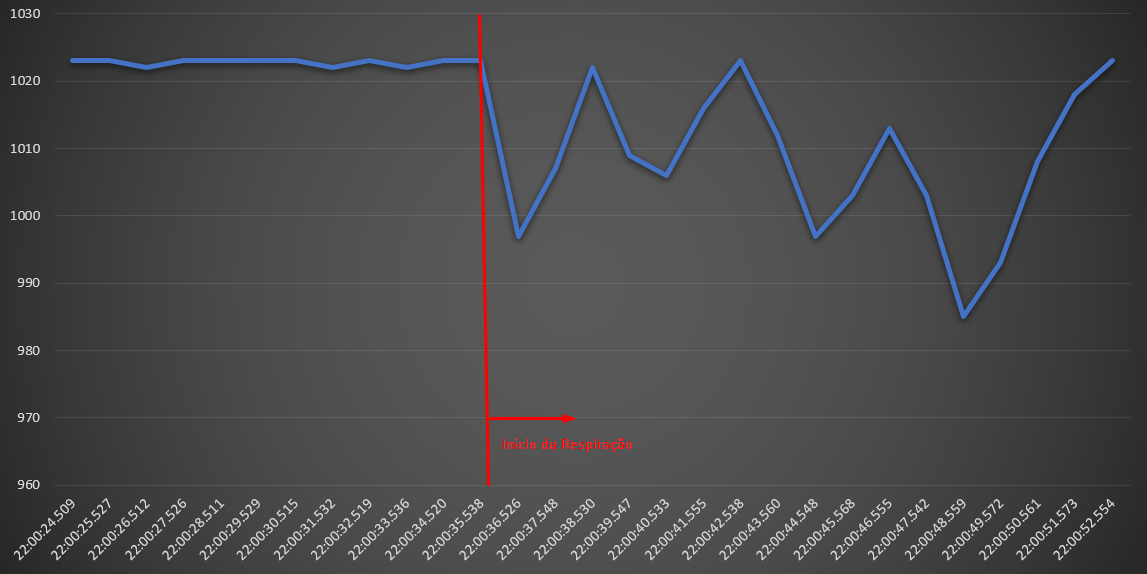
\includegraphics[width=1\linewidth]{images/RespostaCircuitoRealimentado.png}
		\caption{Resposta em curto prazo circuito realimentado (Tempo no eixo horizontal e valor de tensão quantizado no eixo vertical)}
		\label{fig:RespostaCircuitoRealimentado}
	\end{center}
\end{figure}

\begin{figure}[h!]
	\begin{center}
		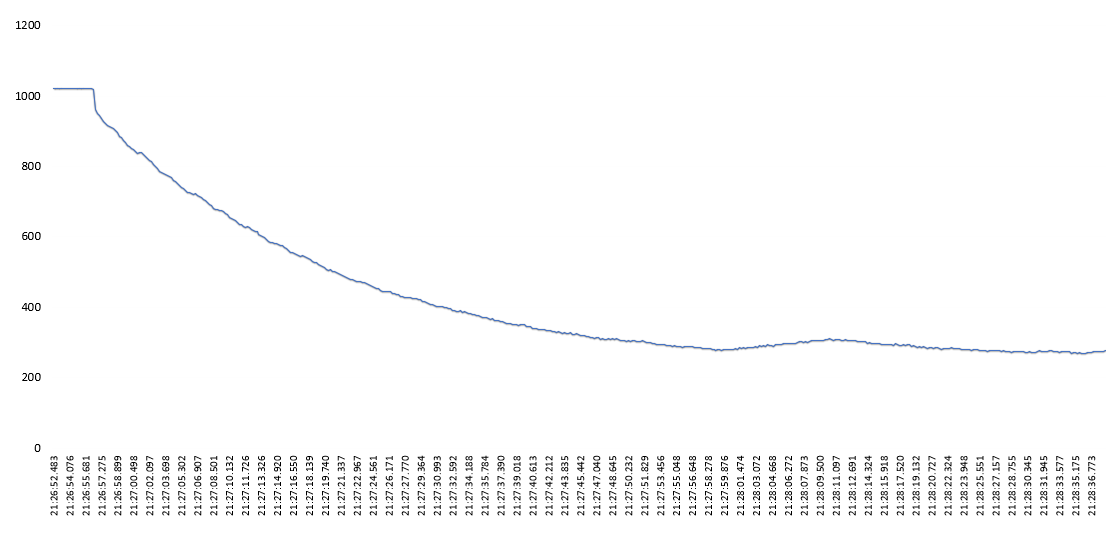
\includegraphics[width=1\linewidth]{images/DecaimentoRespiracaoMascara.png}
		\caption{Resposta de longo prazo circuito realimentado (Tempo no eixo horizontal e valor de tensão quantizado no eixo vertical)}
		\label{fig:RespostaCircuitoRealimentadoLongoPrazo}
	\end{center}
\end{figure}


%\section{A fonte de tensão}
 
 
  
  \include{04_Materiais}

    \chapter{Conclusão}
  
  \section{Contribuições}
  
  \section{Limitações}

  \section{Trabalhos futuros}
  
  \section{Considerações finais}

  \backmatter
  \bibliographystyle{coppe-unsrt}
  \bibliography{example}

  \appendix
  \chapter{Software teste de conceitos}
  
  \begin{figure}[h!]
  	\begin{center}
  		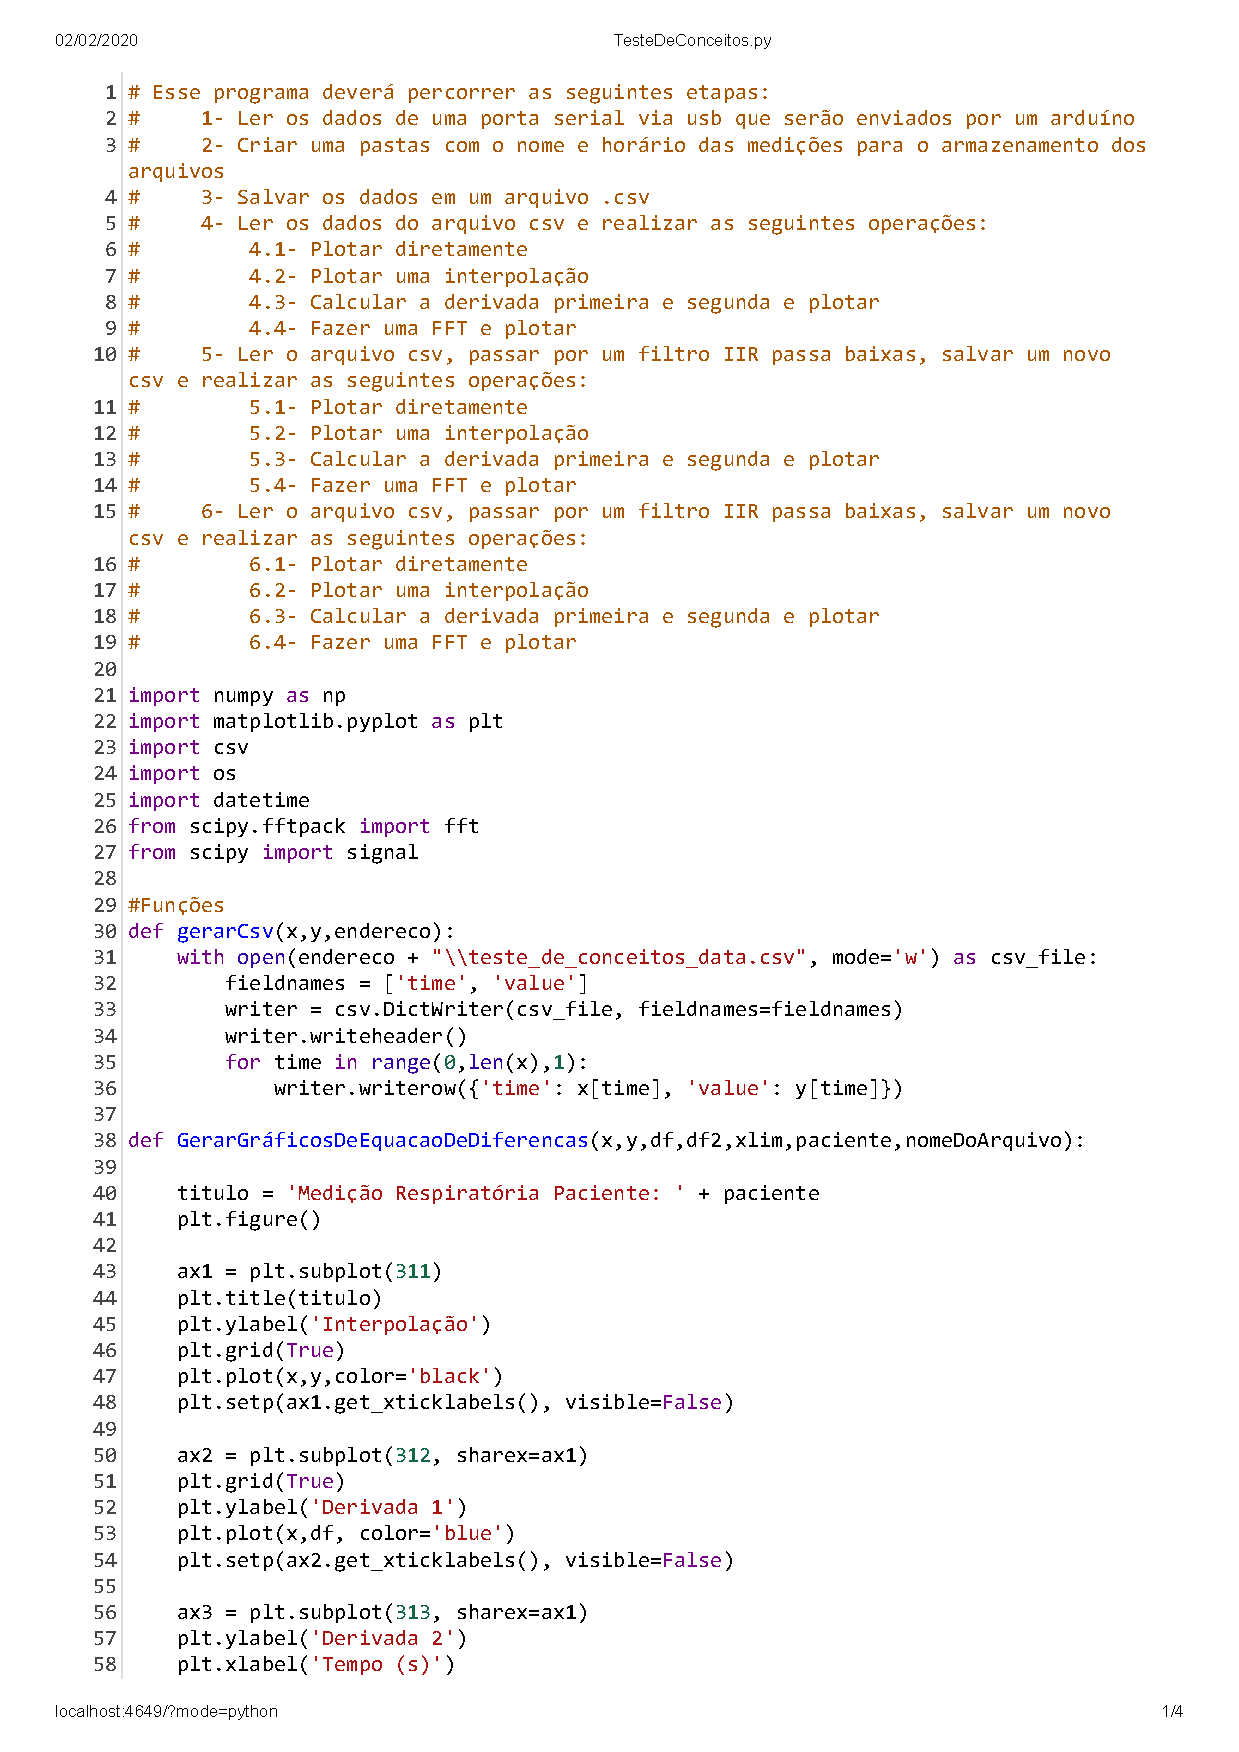
\includegraphics[width=1\linewidth]{images/teste_de_conceitos1.pdf}
  	\end{center}
  \end{figure}
    \begin{figure}[h!]
  	\begin{center}
  		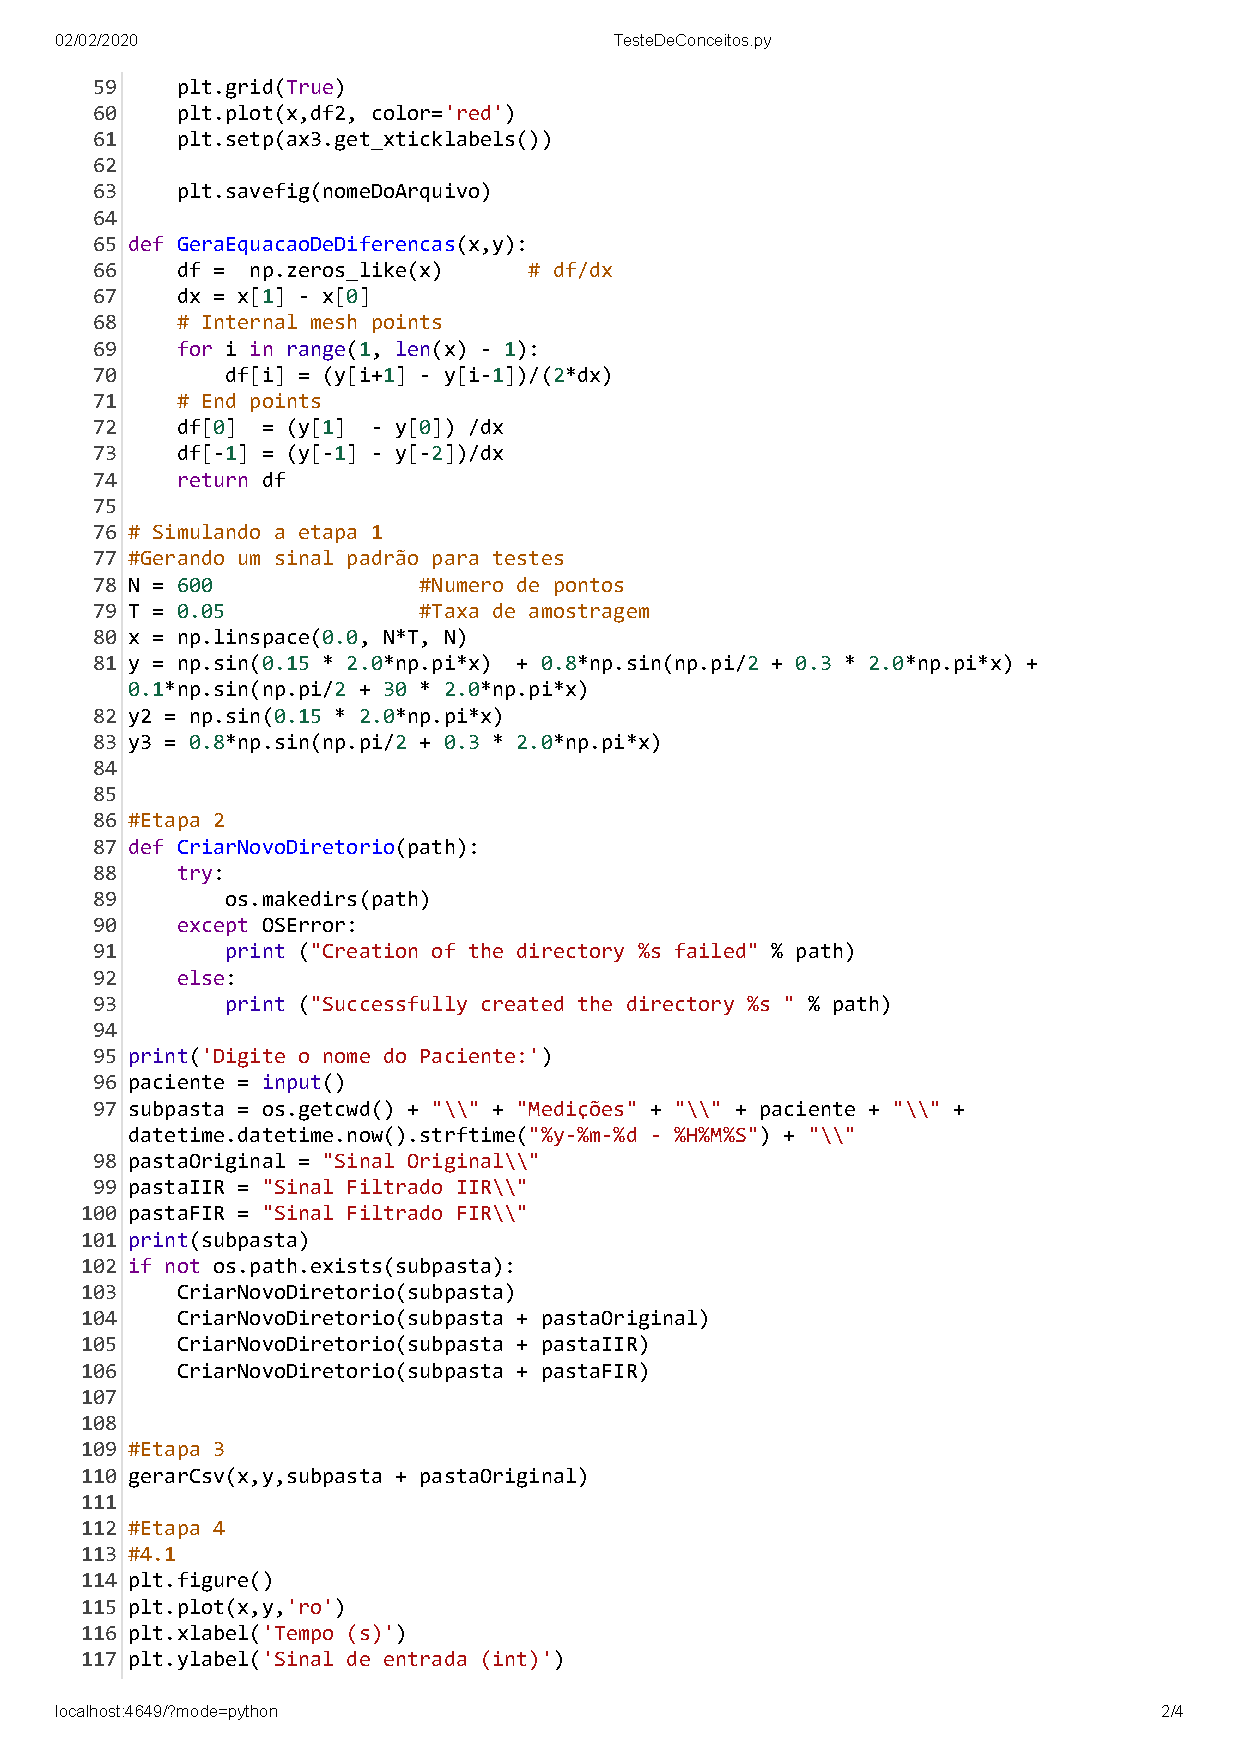
\includegraphics[width=1\linewidth]{images/teste_de_conceitos2.pdf}
  	\end{center}
  \end{figure}
  \begin{figure}[h!]
	\begin{center}
		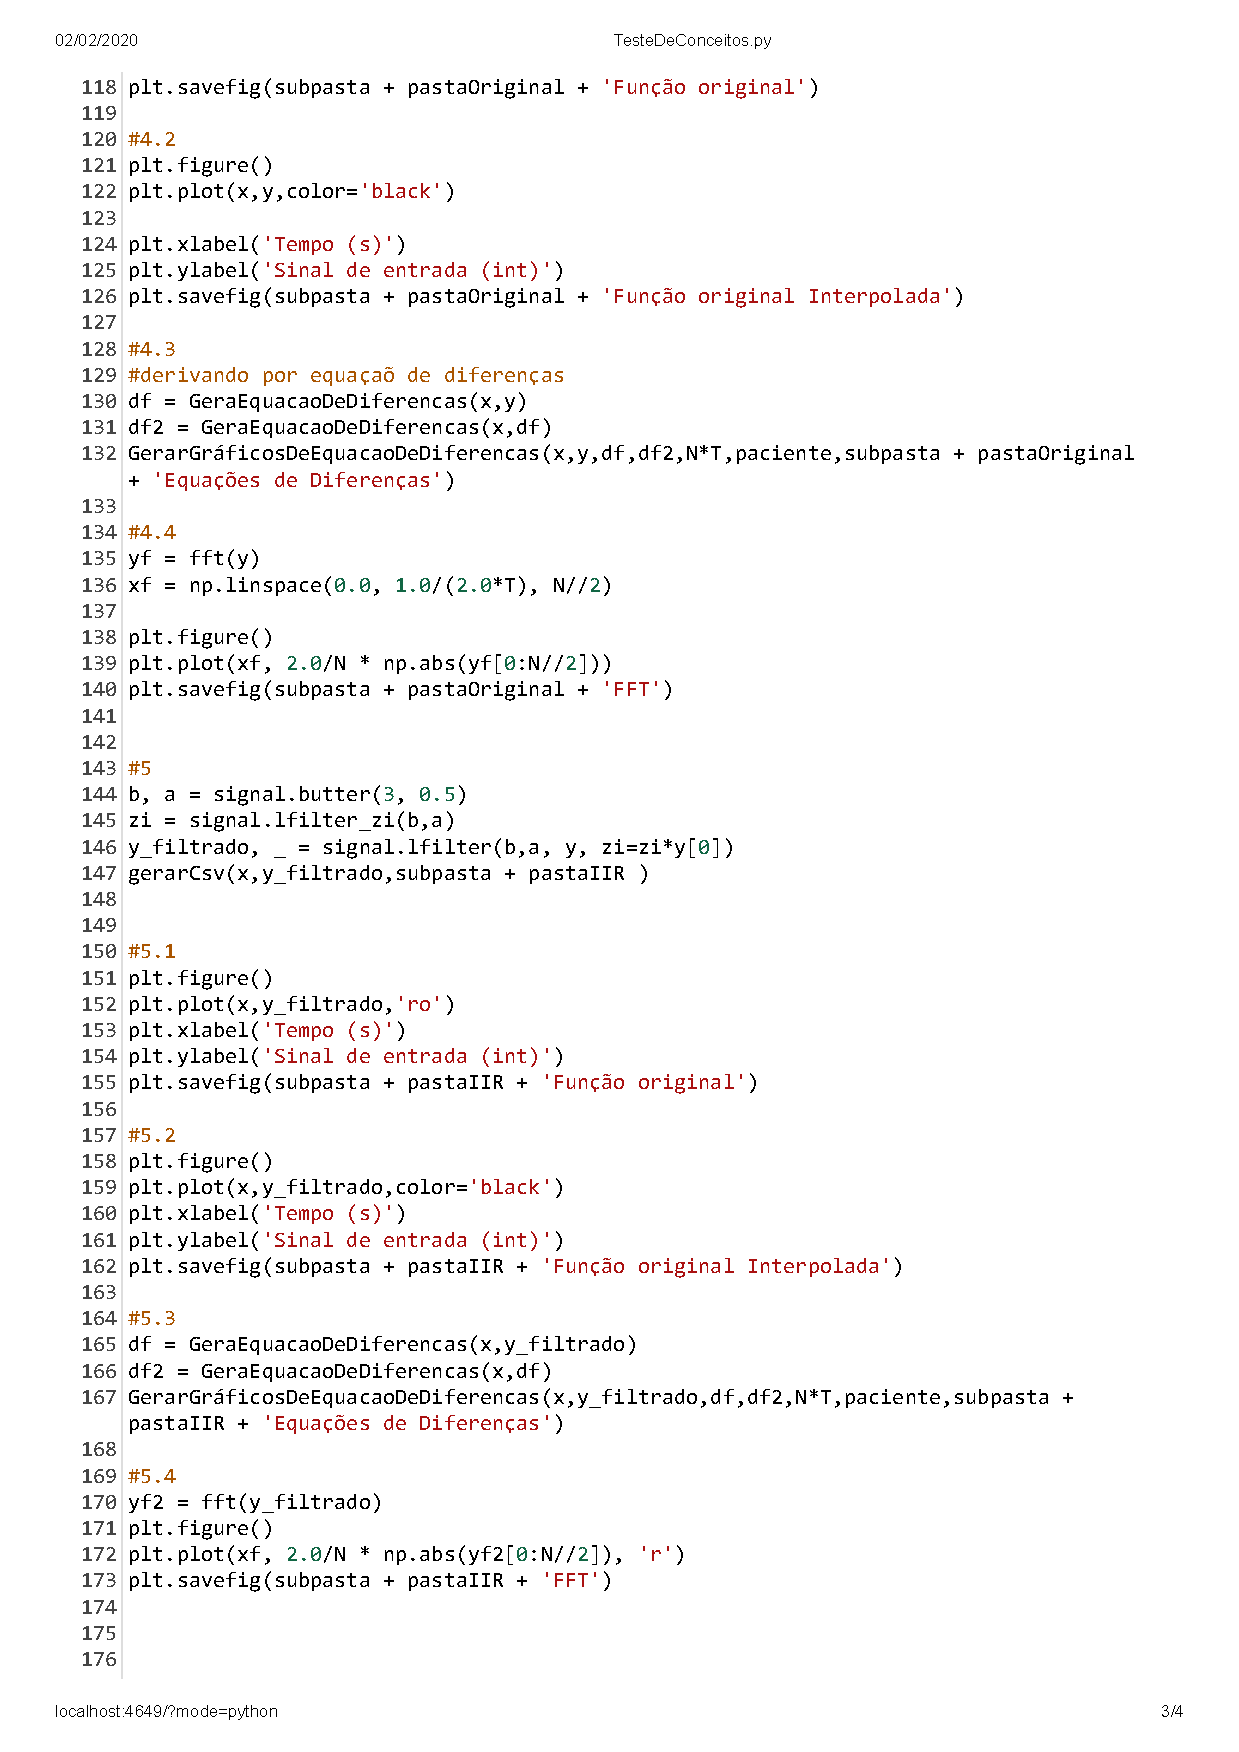
\includegraphics[width=1\linewidth]{images/teste_de_conceitos3.pdf}
	\end{center}
\end{figure}
  \begin{figure}[h!]
	\begin{center}
		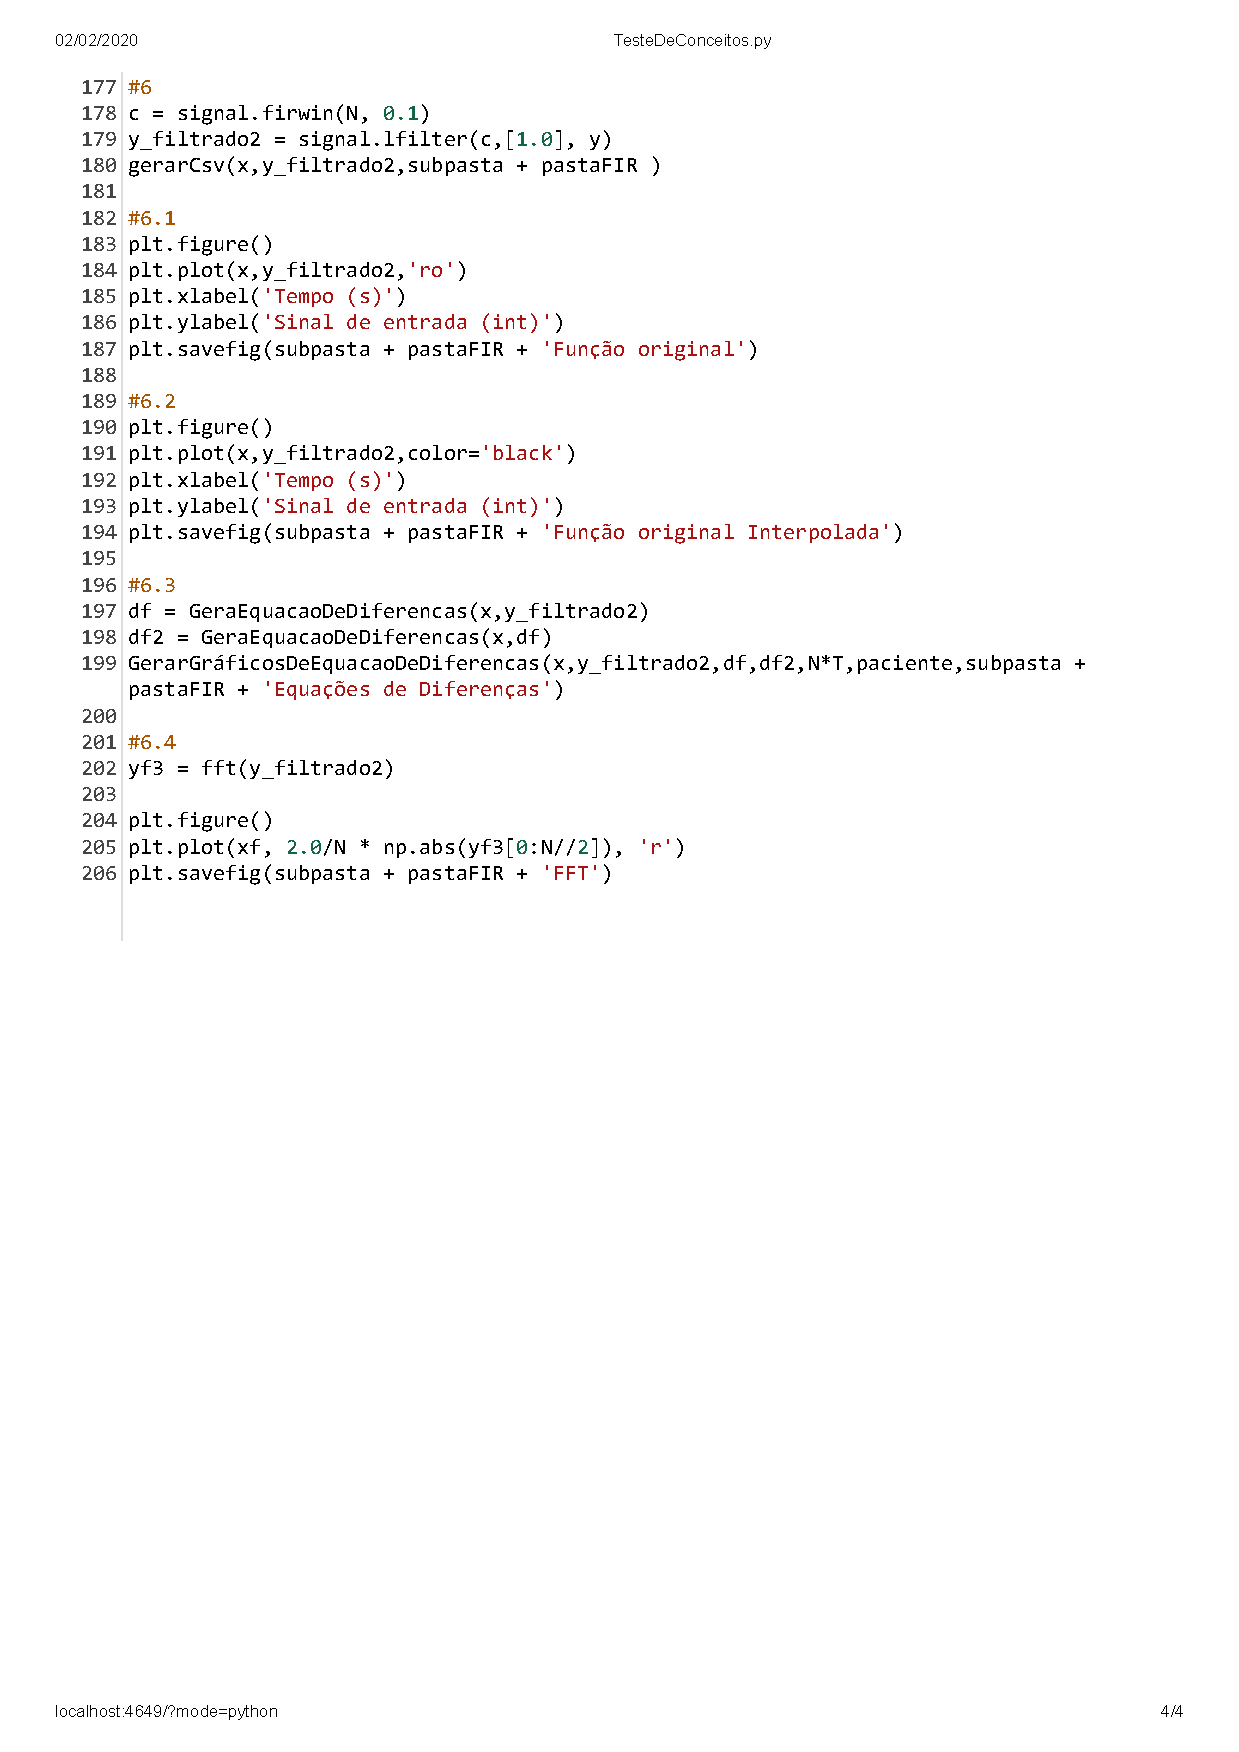
\includegraphics[width=1\linewidth]{images/teste_de_conceitos4.pdf}
	\end{center}
\end{figure}
\end{document}
%% 
%%
%% End of file `example.tex'.
